\documentclass{article}

% if you need to pass options to natbib, use, e.g.:
%     \PassOptionsToPackage{numbers, compress}{natbib}
% before loading neurips_2021

% ready for submission
\usepackage[preprint]{neurips_2021}

% to compile a preprint version, e.g., for submission to arXiv, add add the
% [preprint] option:
%     \usepackage[preprint]{neurips_2021}

% to compile a camera-ready version, add the [final] option, e.g.:
%     \usepackage[final]{neurips_2021}

% to avoid loading the natbib package, add option nonatbib:
%    \usepackage[nonatbib]{neurips_2021}

\usepackage[utf8]{inputenc} % allow utf-8 input
\usepackage[T1]{fontenc}    % use 8-bit T1 fonts
\usepackage[colorlinks=true]{hyperref}       % hyperlinks
\usepackage{url}            % simple URL typesetting
\usepackage{booktabs}       % professional-quality tables
\usepackage{amsfonts}       % blackboard math symbols
\usepackage{nicefrac}       % compact symbols for 1/2, etc.
\usepackage{microtype}      % microtypography
\usepackage{xcolor}         % colors

\usepackage{graphicx}
% package to open file containing variables
\usepackage{datatool, filecontents}
\DTLsetseparator{;}% Set the separator between the columns.

% import data
\DTLloaddb[noheader, keys={thekey,thevalue}]{generalStatistic}{fig/generalStatistic.dat}
% Loads mydata.dat with column headers 'thekey' and 'thevalue'
% \newcommand{\var}[1]{\texttt{\DTLfetch{generalStatistic}{thekey}{#1}{thevalue}}}
\newcommand{\var}[1]{\DTLfetch{generalStatistic}{thekey}{#1}{thevalue}}


\title{A descriptive view on\\ Spotify playlists}

% The \author macro works with any number of authors. There are two commands
% used to separate the names and addresses of multiple authors: \And and \AND.
%
% Using \And between authors leaves it to LaTeX to determine where to break the
% lines. Using \AND forces a line break at that point. So, if LaTeX puts 3 of 4
% authors names on the first line, and the last on the second line, try using
% \AND instead of \And before the third author name.

\author{
  Linus Stenzel\\
  Matrikelnummer 6008798\\
  \texttt{linus.stenzel@student.uni-tuebingen.de} \\
  \And
  Jonas Schmiegel\\
  Matrikelnummer 6002387\\
  \texttt{jonas.schmiegel@student.uni-tuebingen.de} \\
}

\begin{document}

\maketitle

\begin{abstract}
  The aim of this paper is to get an intuition of how Spotify playlists are created and used. We take a look at different key data of playlists e.g. tracks, artists and followers. To cover a wide range of topics we chose a descriptive statistics view. Starting with some general stats, we calculated averages of interesting metrics and show how unique values behave when considering more data. Then we compared popular and unpopular playlists and found differences in the number of unique artists but also in the amount of users that give a description of their playlist.
  
\end{abstract}

\section{Introduction}
Music is an essential part of the human culture. Wherever historians found evidence of human settlement, they also found evidence of musical activities. The oldest discovery of an instrument is a bone flute which is determined to be between 43,000 and 82,000 years old.\citep[p. 63]{Peretz2003} 

One of the biggest companies in today's music industry is Spotify - a streaming service used by hundreds of millions of people.\footnote{In the last shareholder letter of Q4 2021 Spotify announced an active user base of 406 million users.\citep{SpotifyTechnology2022}} Since Spotify has the highest market share ($ \approx 31\% $) in the music industry \citep{Mulligan2022}, we think that our analysis gives an insight of the listening habits of more people than the dataset is representing.
\section{The dataset}

As dataset for our project we are using the \textit{"The Million Playlist Dataset"} \citep{recsysChallenge} from Spotify\footnote{The dataset can be downloaded from \url{https://research.atspotify.com/datasets/}}. It consists of one million playlists (divided into 1,000 JSON files, where each file consist of 1,000 playlists) and is about 34 GB in size. The dataset was sampled from over four billion public playlists on Spotify. It includes only playlists which were created between January 2010 and November 2017 by US Spotify users, that are at least 13 years old. Originally the dataset was introduced as part of the \textit{RexSys Challenge 2018}. The Goal of the \textit{RexSys Challenge 2018} was to create an algorithm suggest appropriate songs to add to a playlist.\footnote{Further information: \url{https://www.recsyschallenge.com/2018/}}

% TODO!!!!
% Add additional constraints the dataset hast (at least 5 tracks in playlist, contains no more than 250 tracks (see line 158 et seq. in the README))

% # Ingnore because it's not necessary
% An example of a playlist in the dataset\footnote{ten tracks are omitted to keep this example small}:
% \inputminted{json}{assets/example.json}
% % \begin{minted}[breaklines, breakanywhere,linenos, numbersep=5pt, gobble=0, frame=single]{json}
% % \end{minted}

% The following list gives a detailed description of the \textit{"The Million Playlist Dataset"} (short MPD).

% \begin{itemize}
%     \item \textbf{name}: Is the name of the playlist\footnote{There are no offensive titles in the dataset. In addition to this adult-oriented titles were excluded when the are created by a user under 18 years}
%     \item \textbf{pid}: Is an id (integer between 0 and 999,999) for the playlist in the MPD
%     \item \textbf{collaborative}: True if the playlist is a collaborative playlist, where multiple users may have added tracks to the playlist
%     \item \textbf{modified\_at}: Timestamps (in seconds since the epoch and rounded to midnight GMT of the date) when the playlist was modified
%     \item \textbf{num\_albums}: Number of unique albums for the tracks in the playlist
%     \item \textbf{num\_tracks}: Number of tracks in the playlist
%     \item \textbf{num\_followers}: Number of followers of the playlist\footnote{Not included is the playlist creator. Also is the number from the time, where the MPD was created.}
%     \item \textbf{num\_edits}: Number of separate editing sessions\footnote{Editing session are separated by a two-hour window in which no other track has been added.}
%     \item \textbf{duration\_ms}: The total duration of all the tracks in the playlist (in milliseconds)
%     \item \textbf{num\_artists}: Number of unique artist for thee tracks in the playlist
%     \item \textbf{tracks}: An array of infromation about all tracks in the playlist. Each entry has the following informations
%     \begin{itemize}
%         \item \textbf{pos}: Position of the track in the playlist\footnote{the first position is considert to be 0}
%         \item \textbf{artists\_name}: The name of the track's primary artist
%         \item \textbf{track\_uri}: The Spotify URI of the track
%         \item \textbf{artist\_uri}: The Spotify URI of the track's primary artist
%         \item \textbf{track\_name}: The name of the track
%         \item \textbf{album\_uri}: The Spotify URI of the album
%         \item \textbf{duration\_ms}: The duration of the track (in milliseconds)
%         \item \textbf{album\_name}: The name of the album
%     \end{itemize}
% \end{itemize}

\section{General Statistics}
To get a broad overview of the dataset we decided to make some general numerical analysis of the dataset to get a feeling for Spotify playlists as data and the scope of the dataset. In the part of the dataset that we are analyzing there are \var{SizeDataset} playlists\footnote{Originally there are 1 million playlists. Due to limited processing power we had to reduce our analysis to a dataset of \var{SizeDataset} playlists.} with a total number of \var{unique_tracks} unique tracks by \var{artists_unique} artists in \var{albums_unique} albums. The total length of all playlist is \var{converted_total_duration} (hrs.:min.:sec.).

The average number of tracks in one playlist are $\approx$ \var{approx_average_numtracks}\footnote{The exact number are \var{average_numtracks} tracks} tracks. Figure \ref{fig:averagetrack} shows how the average number of tracks per playlists changes, when more and more playlists are considered. 

\begin{figure}[ht]
    \centering
    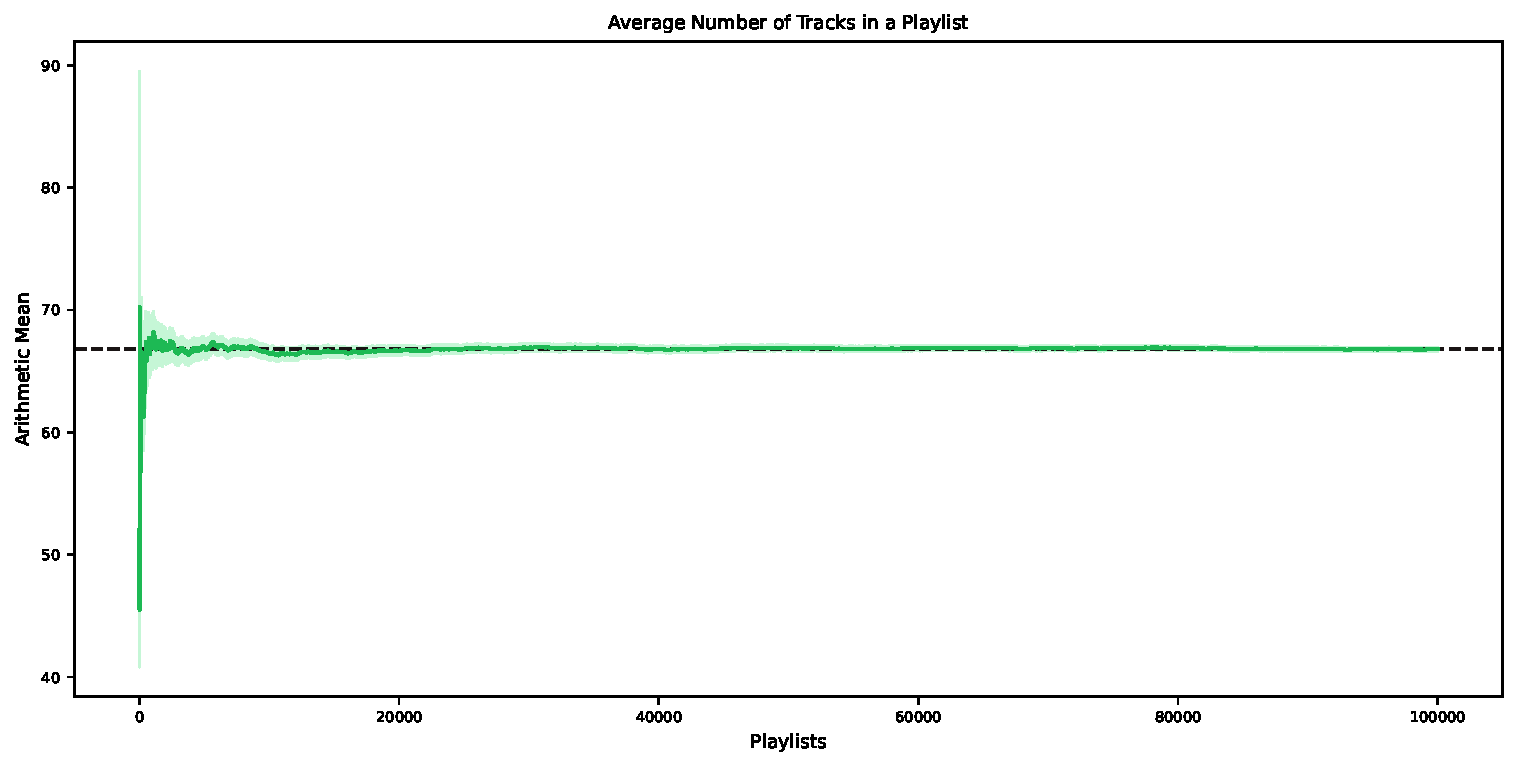
\includegraphics[width=\textwidth]{fig/averageTrack.pdf}
    \caption{CAPTION}
    \label{fig:averagetrack}
\end{figure}

The average duration of a playlist is \var{converted_average_duration}. This fits (approximately) with the fact, that a track has an average duration of \var{converted_average_track_duration}.\footnote{Using the following calculation:\\$\text{average duration of track [ms]}\cdot\text{average number of tracks in a playlist}=\var{average_track_duration} \text{ ms}\cdot\var{average_numtracks}= \var{cal_average_playlist_duration} \text{ ms} = $ \var{converted_cal_average_playlist_duration}}

Knowing the average number of tracks per playlist, we wanted to know how much any new playlist contributes to this. For that we looked how the number of unique tracks changes when considering more playlists and plotted the results. To clearly show the relation we changed the x-axis to a square root scale.

\begin{figure}[ht]
    \centering
    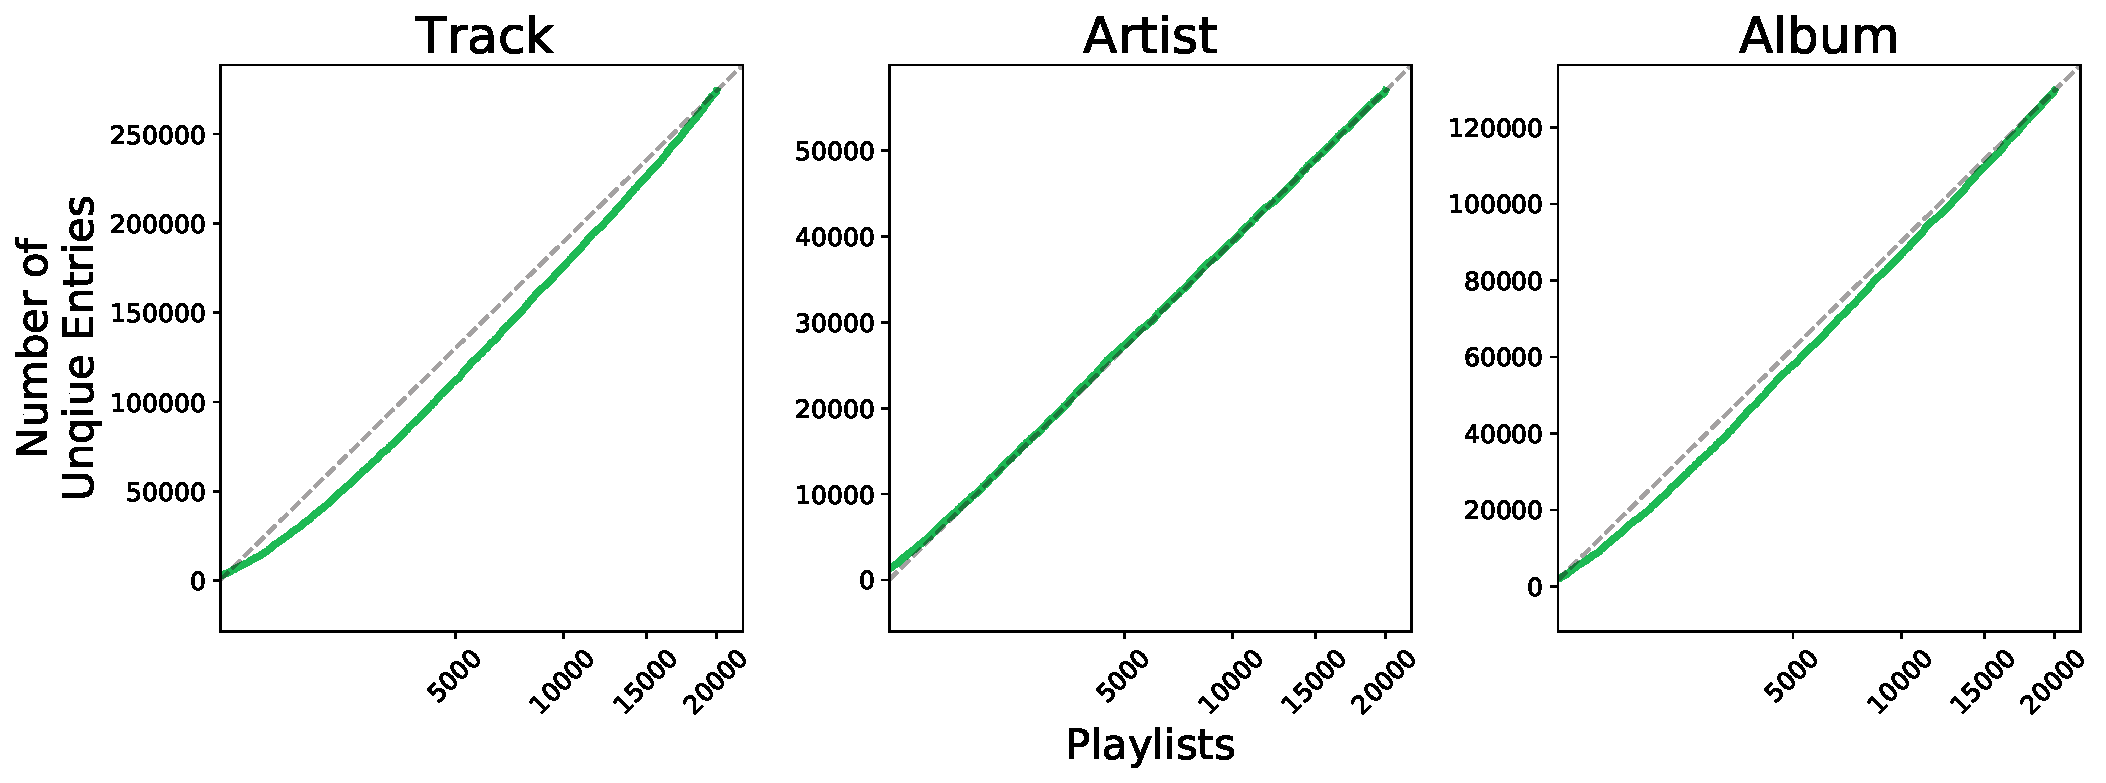
\includegraphics[width=\textwidth]{fig/unique_to_playlist.pdf}
    \caption{Line plot showing the relation between e.g. unique tracks and considered playlists}
    \label{fig:unique_to_playlist}
\end{figure}

We now know that the first $n$ playlists contribute the same amount of unique tracks as the $n^2$ playlist after. The same holds for artists and albums.


To get the most popular tracks, albums and artists, we counted how often they were occurring in a playlist. The result is shown in tab. \ref{tab:popular}. The top 15 tracks are expectedly matching with the first 15 billboard charts of 2017.\citep{BillboardMedia}

\begin{table}[]
    \centering
    \caption{CAPTION}
    \begin{tabular}{clllllllll} \toprule
    Pos. & Occur.               & Track                 & Occur.               & Album                 & Occur.                & Artist                 \\
    \midrule
    1   & \var{top1track_occ}  & \var{top1track_name}  & \var{top1album_occ}  & \var{top1album_name}  & \var{top1artist_occ}  & \var{top1artist_name}  \\
    2   & \var{top2track_occ}  & \var{top2track_name}  & \var{top2album_occ}  & \var{top2album_name}  & \var{top2artist_occ}  & \var{top2artist_name}  \\
    3   & \var{top3track_occ}  & \var{top3track_name}  & \var{top3album_occ}  & \var{top3album_name}  & \var{top3artist_occ}  & \var{top3artist_name}  \\
    4   & \var{top4track_occ}  & \var{top4track_name}  & \var{top4album_occ}  & \var{top4album_name}  & \var{top4artist_occ}  & \var{top4artist_name}  \\
    5   & \var{top5track_occ}  & \var{top5track_name}  & \var{top5album_occ}  & \var{top5album_name}  & \var{top5artist_occ}  & \var{top5artist_name}  \\
    6   & \var{top6track_occ}  & \var{top6track_name}  & \var{top6album_occ}  & \var{top6album_name}  & \var{top6artist_occ}  & \var{top6artist_name}  \\
    7   & \var{top7track_occ}  & \var{top7track_name}  & \var{top7album_occ}  & \var{top7album_name}  & \var{top7artist_occ}  & \var{top7artist_name}  \\
    8   & \var{top8track_occ}  & \var{top8track_name}  & \var{top8album_occ}  & \var{top8album_name}  & \var{top8artist_occ}  & \var{top8artist_name}  \\
    9   & \var{top9track_occ}  & \var{top9track_name}  & \var{top9album_occ}  & \var{top9album_name}  & \var{top9artist_occ}  & \var{top9artist_name}  \\
    10  & \var{top10track_occ} & \var{top10track_name} & \var{top10album_occ} & \var{top10album_name} & \var{top10artist_occ} & \var{top10artist_name} \\
    11  & \var{top11track_occ} & \var{top11track_name} & \var{top11album_occ} & \var{top11album_name} & \var{top11artist_occ} & \var{top11artist_name} \\
    12  & \var{top12track_occ} & \var{top12track_name} & \var{top12album_occ} & \var{top12album_name} & \var{top12artist_occ} & \var{top12artist_name} \\
    13  & \var{top13track_occ} & \var{top13track_name} & \var{top13album_occ} & \var{top13album_name} & \var{top13artist_occ} & \var{top13artist_name} \\
    14  & \var{top14track_occ} & \var{top14track_name} & \var{top14album_occ} & \var{top14album_name} & \var{top14artist_occ} & \var{top14artist_name} \\
    15  & \var{top15track_occ} & \var{top15track_name} & \var{top15album_occ} & \var{top15album_name} & \var{top15artist_occ} & \var{top15artist_name} \\
    \bottomrule
    \end{tabular}
    \label{tab:popular}
\end{table}
\section{Characteristics of Mainstream Playlists}
We analyzed the difference between playlists that contain an above-average amount of mainstream tracks and playlists that contain mostly uncommon tracks. For this we first had to establish a measurement from which we can identify a playlist as mainstream. As previously described we have calculated the most common tracks. We determined an arbitrary but reasonable border, which is to contain at least three of the top 50 common tracks to count as a mainstream playlist. To obtain the same group sizes between mainstream and uncommon playlists, we sampled from the larger one (uncommon playlist). We then looked for differences between the groups and found that playlists with popular tracks have less unique artists than playlists with unpopular tracks. 

\begin{figure}[ht]
    \centering
    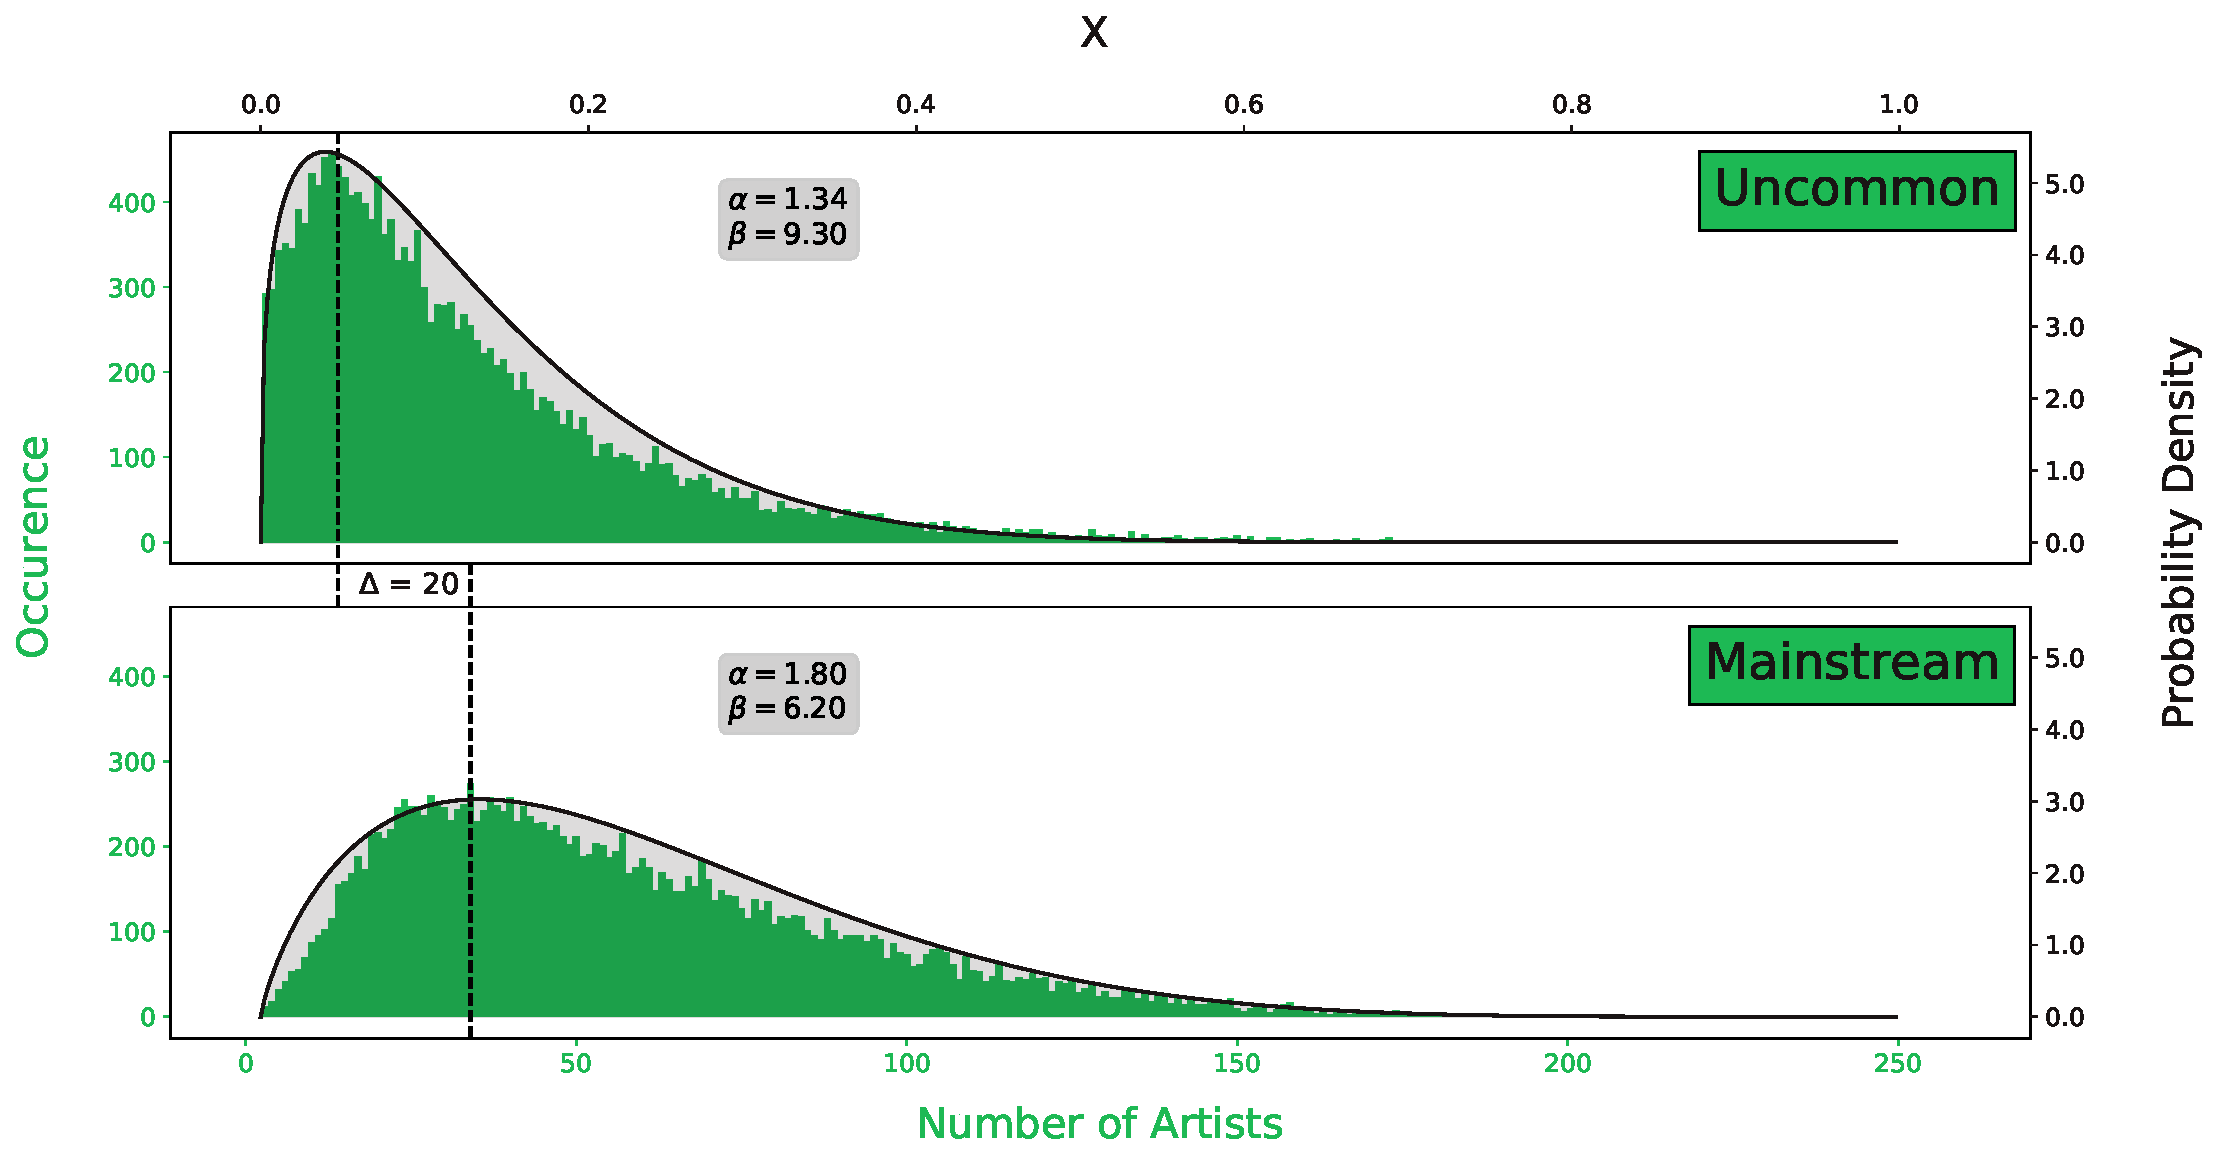
\includegraphics[width=\textwidth]{fig/pop_unpop_artist.pdf}
    \caption{Histogram of Number of Artists (\textcolor{spotifygreen}{---}) with fitted Beta distribution (\textcolor{black}{---}) for uncommon and mainstream playlists}
    \label{fig:pop_unppo_artist}
\end{figure}

To show this we plotted the number of artists against its occurrence for both groups. Just by looking at the mode (Uncommon=14; Mainstream=34) we can see that there is a difference but to further underlie our finding we fitted a beta distribution to the data. The input values of a beta distribution are between 0 and 1. Since the playlists in the dataset are constrained to have at least three but no more than 250 artists, also the data has limits on both sides. The probability density of both beta distributions is shifted to the lower border. We can see that the beta distribution of uncommon playlists has nearly all of its mass around the mode, while the mass of the beta distribution of mainstream playlists is much more spread.

We also thought of metric that can directly measure the popularity of a playlist, which is the number of followers of a playlist. The playlists are constrained to have at least one follower and more than 90\% of the playlist have three or less. This is why we decided to not split the data into the binary groups, popular and unpopular. Nevertheless, we found that the more follower a playlist has, the more likely it is for the playlist to have a description.

\begin{figure}[ht]
    \centering
    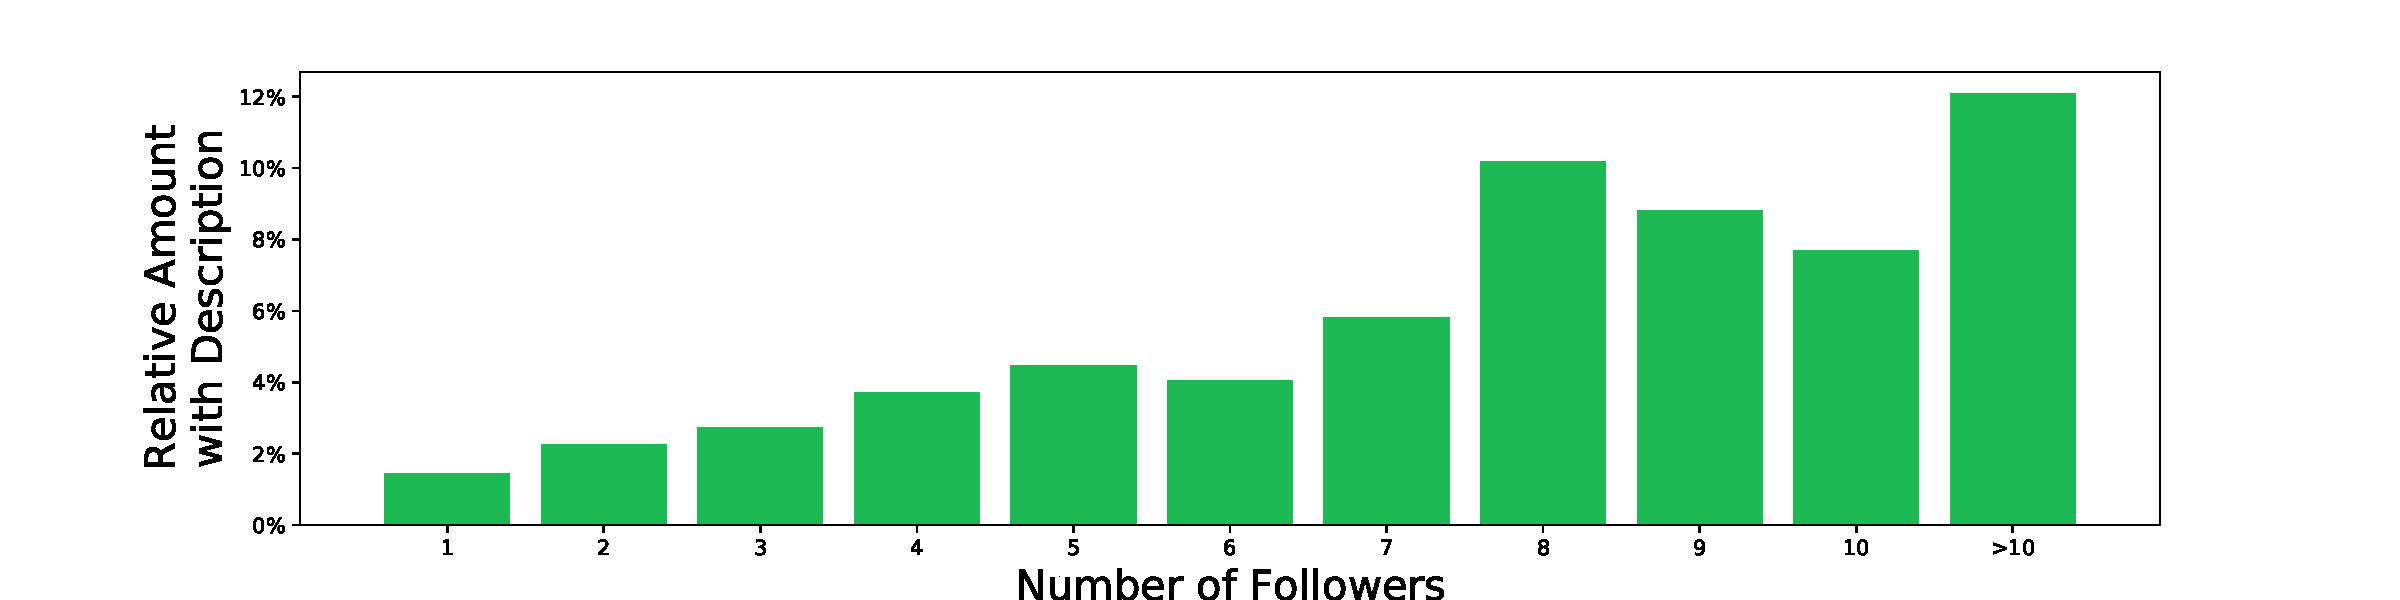
\includegraphics[width=\textwidth]{fig/followers_to_description.pdf}
    \caption{Bar plot of number of followers to relative amount with description}
    \label{fig:followers_to_description}
\end{figure}

We grouped the playlists by their follower number and counted the ones that have been given a description. Because the groups heavily differ in size, we calculated the relative amount. As mentioned, the data pool for playlists with higher follower numbers gets very small. That is why we put all playlists with more than ten followers into a single group.

\bibliography{bibliography}
% \bibliography{sample}

\end{document}